\section{Direct optimisation of PSYCHE waveform}
\label{sec:pureshift__optimisation}

The changes to the PSYCHE waveform discussed in the previous section---changing the number of saltire pulses to either 1 or 4---are fairly minor, in that they do not fundamentally alter the form of the PSE.
Furthermore, there is an obvious issue in that the quality of the spectrum is not measured in a particularly rigorous manner.
Ideally, we would like to have a mathematical way of measuring how well the pure shift sequence has worked.
Such a metric would also enable a more automated optimisation process, where a programme is allowed to find the best PSE without any interference from human subjectivity.

In this section, I discuss more radical changes which depart from the tried-and-tested saltire pulse.
I also show how two different \textit{cost functions}---functions which determine how `bad' a spectrum is---can be used to evaluate PSEs.
Although the work in this section did not quite yield any groundbreaking results, it provided substantial insights into the nature of pure shift optimisations, which were later used in the context of POISE (\cref{chpt:poise}).

\subsection{Techniques for pure shift optimisations}
\label{subsec:pureshift__optim_techniques}

Throughout this chapter (and more generally this thesis), various algorithms are used for \textit{optimisation}: that is, to find the parameters $\symbf{x} \in \mathbb{R}^n$ which minimise a \textit{cost function} $f : \mathbb{R}^n \to \mathbb{R}$.
The theory of optimisation is covered in more detail in \cref{sec:poise__introduction}, so will not be repeated now.
Here, I make a distinction only between \textit{derivative-based} and \textit{derivative-free} optimisation algorithms: the former use extra information in the form of $\nabla f$ to help locate the optimum, whereas the latter do not, using only the value of $f(\symbf{x})$.
While derivative-based algorithms typically converge to an optimum more quickly, they are unsuitable for problems where the cost function $f$ is noisy.
In this section, the Nelder--Mead (NM) simplex algorithm\autocite{Nelder1965TCJ} was used: it is a very popular derivative-free method, and although mathematical convergence is not guaranteed\autocite{McKinnon1998SIAMJO}, in practice such cases are rather unlikely to arise.
In this section, the implementation of the NM algorithm in the Python \texttt{scipy} package was simply used as-is.

The cost function measuring the performance of a pure shift experiment can be measured in one of two ways: either \textit{theoretically}, in that the pure shift experiment is simulated using the density operator formalism, or \textit{experimentally}, in that the experiment is run on a spectrometer.
Unfortunately, the simulation of PSYCHE-type PSEs, where a shaped pulse is applied together with a gradient, requires a large amount of time.
The pulse itself already has $n \sim 10000$ points, but on top of that, the application of gradients also requires splitting up the sample into multiple slices (often 100 to 1000) such that the evolution of $\rho$ can be simulated in each slice and the results summed up.
To make matters worse, $H_\text{pulse}$ does not commute with $H_\text{grad}$, so a propagator
\begin{equation}
    \label{eq:pulse_gradient_propagator}
    U(i, z) = \exp\left[-\mi(H_\text{grad}(z) + H_\text{free} + c_x^{(i)}I_x + c_x^{(i)} I_y)(\delta t)\right]
\end{equation}
must be calculated for each pulse point ($1 \leq i \leq n$) in each slice of the sample.
As a result, the simulation of PSYCHE spectra in the Spinach package\Autocite{Hogben2011JMR} typically requires minutes to hours.%
\footnote{With highly optimised handwritten code, exploiting the symmetry of the PSYCHE element, the fastest simulation I could do took 16 seconds on a 20-core computer, for a simple 2-spin system. This number increases very rapidly for larger spin systems. It is possible that GPU acceleration could result in substantial speedups, but I have not looked into this sufficiently. Anyway, acquisition of the pure shift spin echo experiment takes only around 5 seconds.}

This in fact makes it faster to experimentally acquire a pure shift spectrum and calculate a cost function based on that.
Running an actual pure shift experiment, though, is suboptimal: firstly, the pseudo-2D interferogram method is slow, and secondly, there is no easy way to devise a cost function for the resulting spectrum.
Instead, we can use a simple 1D `pure shift spin echo' (PSSE) sequence, which has the form \ang{90}--$\tau$--PSE--$\tau$--detect (\cref{fig:psse_psse}).
An ideal PSE would lead to complete refocusing of both chemical shifts and J-couplings, and the signal detected after this would simply be the same as in a pulse--acquire experiment (\cref{fig:psse_zg}).
Of course, there is a sensitivity penalty which reflects that of the PSE.
On top of that, if the J-refocusing is not perfect, then the multiplets in the spin echo sequence acquire a degree of phase distortion: the delay $\tau$ has to be long enough to allow for this, but its exact value is otherwise largely insignificant.
These distortions are just about visible in \cref{fig:psse_psse}.

\begin{figure}[htbp]
    \centering
    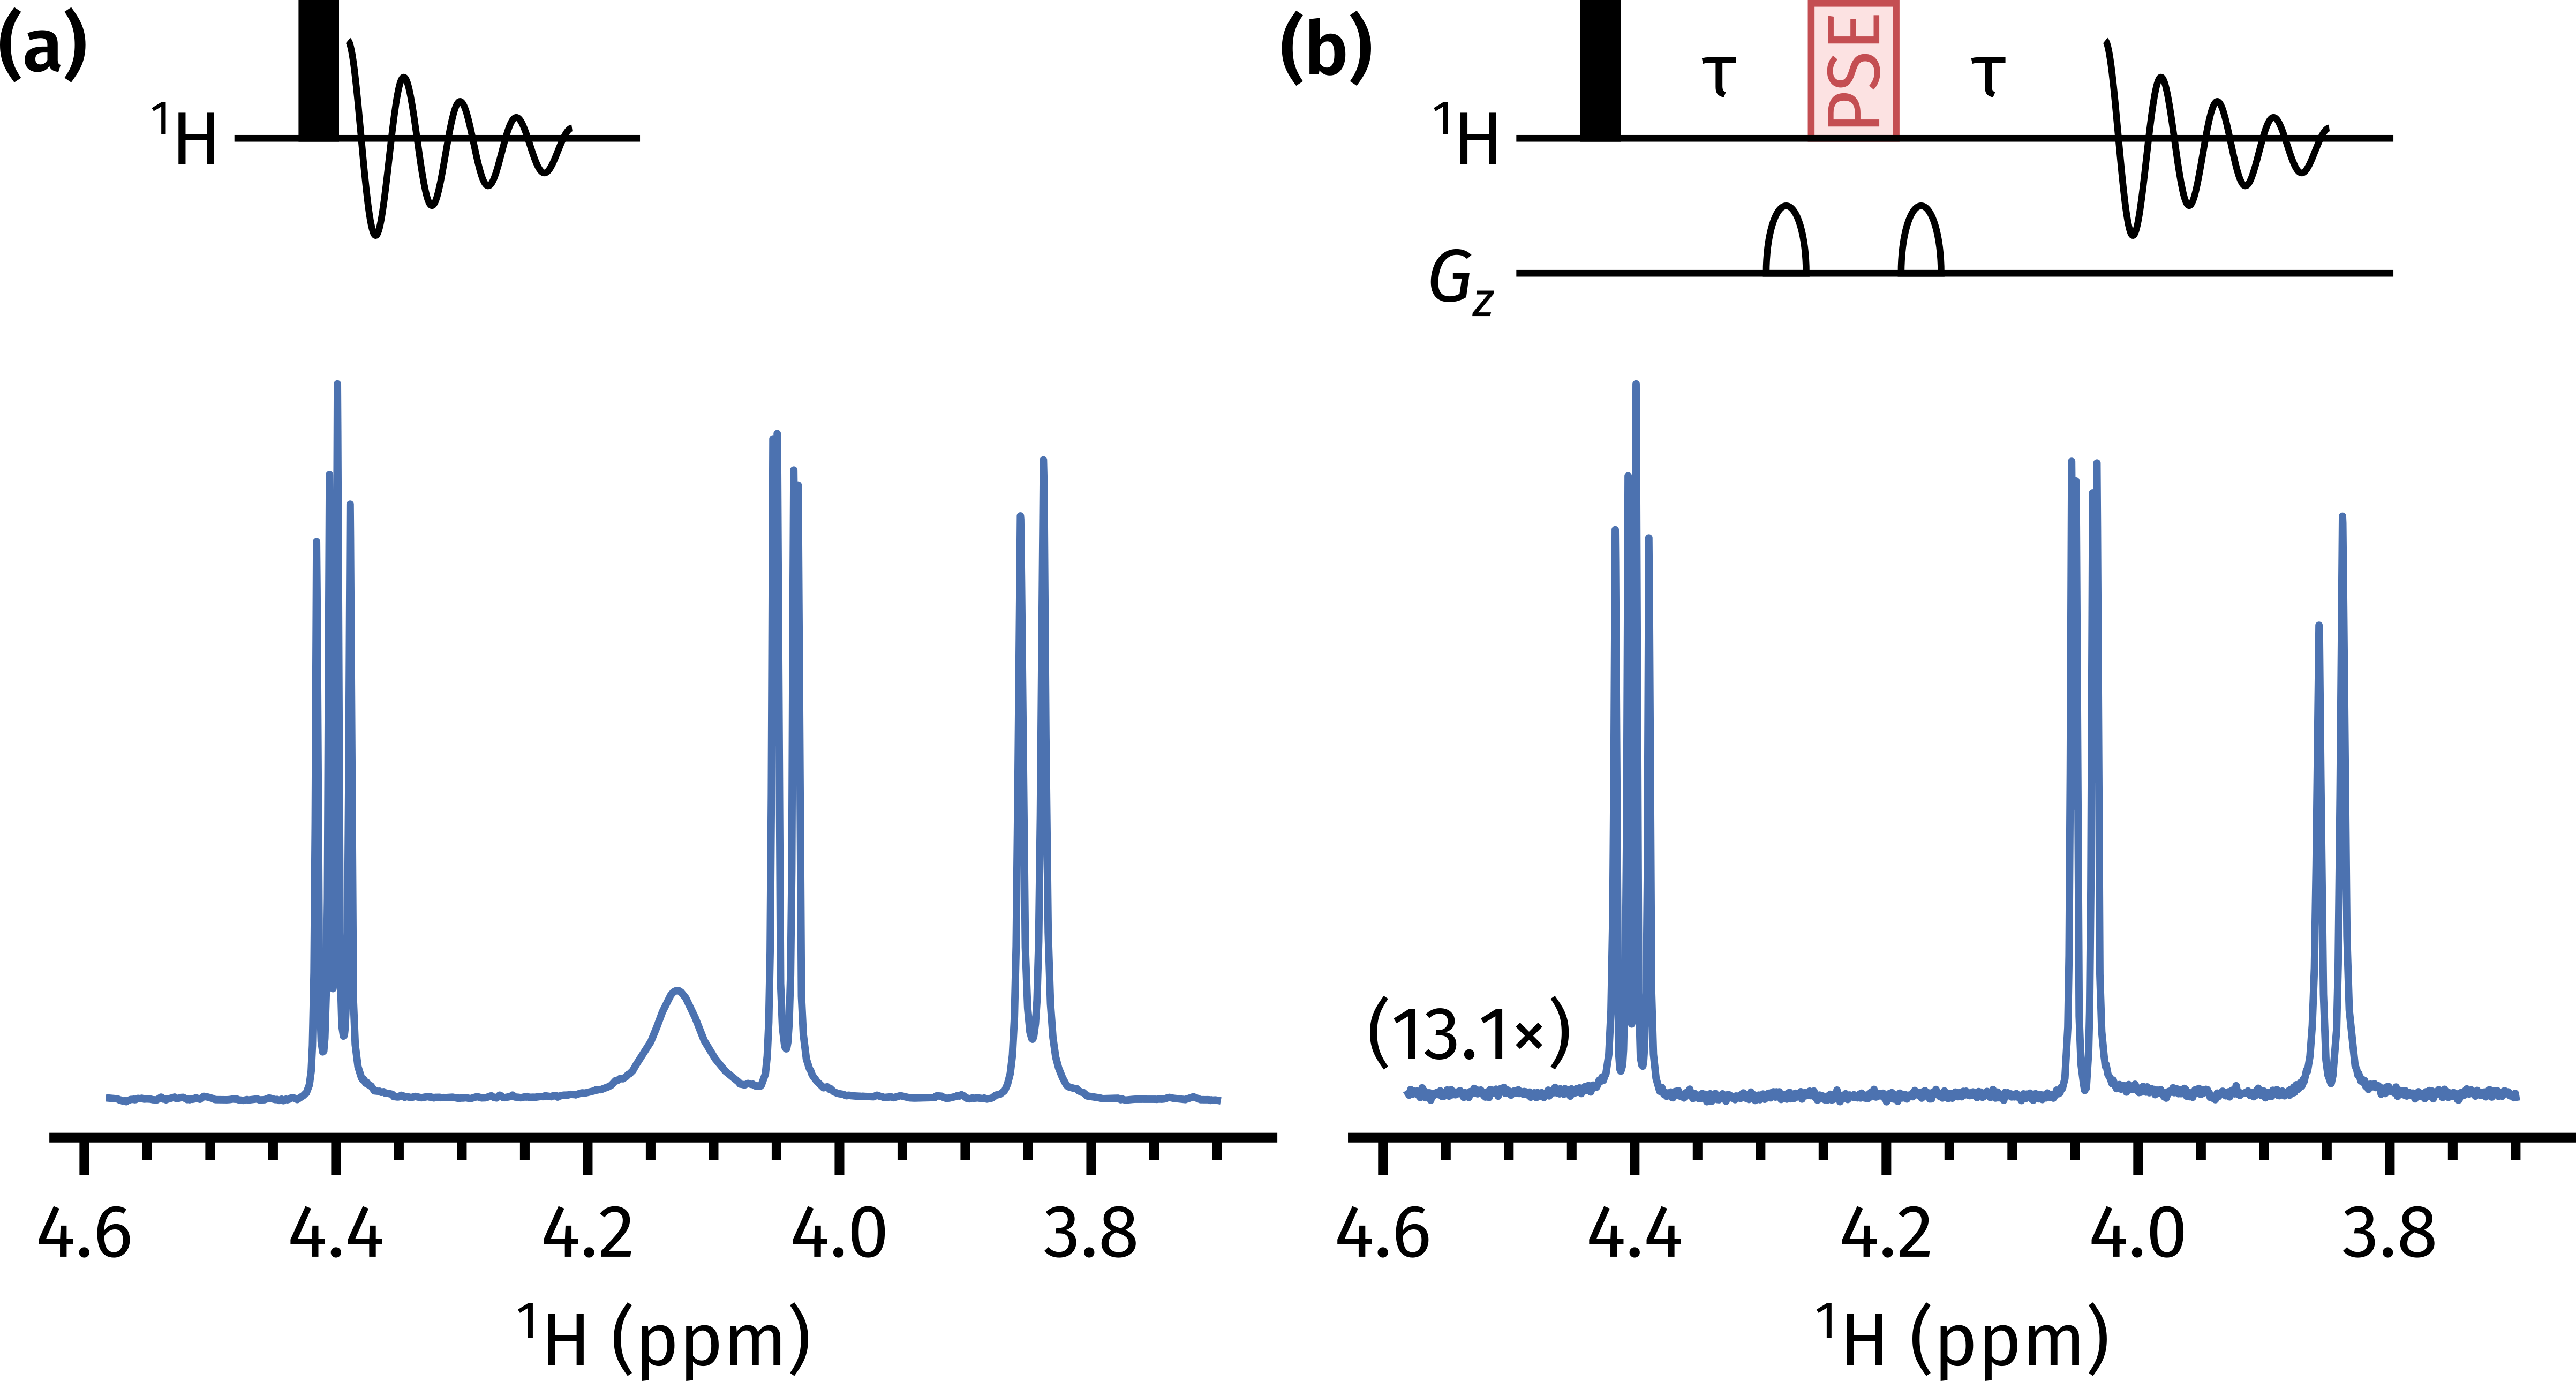
\includegraphics[]{pureshift/psse.png}
    {\phantomsubcaption\label{fig:psse_zg}}
    {\phantomsubcaption\label{fig:psse_psse}}
    \caption[Pure shift spin echo experiment]{
        \textbf{(\subref{fig:psse_zg})} Pulse--acquire experiment and the resulting spectrum.
        \textbf{(\subref{fig:psse_psse})} Pure shift spin echo experiment and the resulting spectrum.
        The PSE used was the PSYCHE double saltire, with a flip angle of \ang{25}; the delay $\tau$ was \SI{11}{\ms}.
        The OH peak at \SI{4.1}{ppm} is lost, most likely due to chemical exchange.
        \datacode{6A-200816}
    }
    \label{fig:ps_optim}
\end{figure}

Two cost functions were designed and used in this section:
\begin{align}
    f_\text{phase} &= \Var_i\left[\arctan\left(\frac{S_{\text{re},i}}{|S_{\text{im},i}|}\right)\right] \label{eq:ps_cf_phase} \\
    f_\text{diff} &= \Biggl\lVert \frac{\symbf{S}_\text{re}}{\lVert \symbf{S}_\text{re} \rVert} - \frac{\symbf{T}_\text{re}}{\lVert \symbf{T}_\text{re} \rVert} \Biggr\rVert, \label{eq:ps_cf_diff}
\end{align}
where the PSSE and pulse--acquire 1D spectra are treated as complex-valued vectors $\symbf{S}$ and $\symbf{T}$ respectively (for \textit{`spectrum'} and \textit{`target'}). $\symbf{S}_\text{re}$ and $\symbf{S}_\text{im}$ are the real and imaginary parts of the spectrum $\symbf{S}$, and $S_{\text{re},i}$ is the $i$-th point of the real part of the spectrum.
The operator $\Var_i$ represents the variance over all points in the spectrum $i$, and $\lVert \symbf{x} \rVert$ denotes the 2-norm of the vector $\symbf{x}$, i.e.\ $\sqrt{\sum_i x_i^2}$.
The implementation of this in Python (\cref{lst:pureshift_costfunctions}) is quite possibly easier to take in.\footnote{The use of \texttt{np.arctan} (the arctangent), and \textit{not} \texttt{np.arctan2} (the argument of a complex number), is intentional. The behaviour shown in \cref{fig:fa_scan_synthetic} isn't reproduced with \texttt{arctan2}. Of course, this means the name `phase' is a misnomer; it's not really the phase of anything meaningful.}

\begin{mylisting}[htb]
\begin{tcbminted}{python}
import numpy as np
# assume S and T are complex numpy arrays which have been read in
Sr = np.real(S); Si = np.imag(S); Tr = np.real(T)
f_phase = np.var(np.arctan(Sr / np.abs(Si)))
f_diff = np.linalg.norm((Sr / np.linalg.norm(Sr))
                        - (Tr / np.linalg.norm(Tr)))
\end{tcbminted}
    \caption[Pure shift cost functions]{Pure shift cost functions.}
    \label{lst:pureshift_costfunctions}
\end{mylisting}

\begin{figure}[htb]
    \centering
    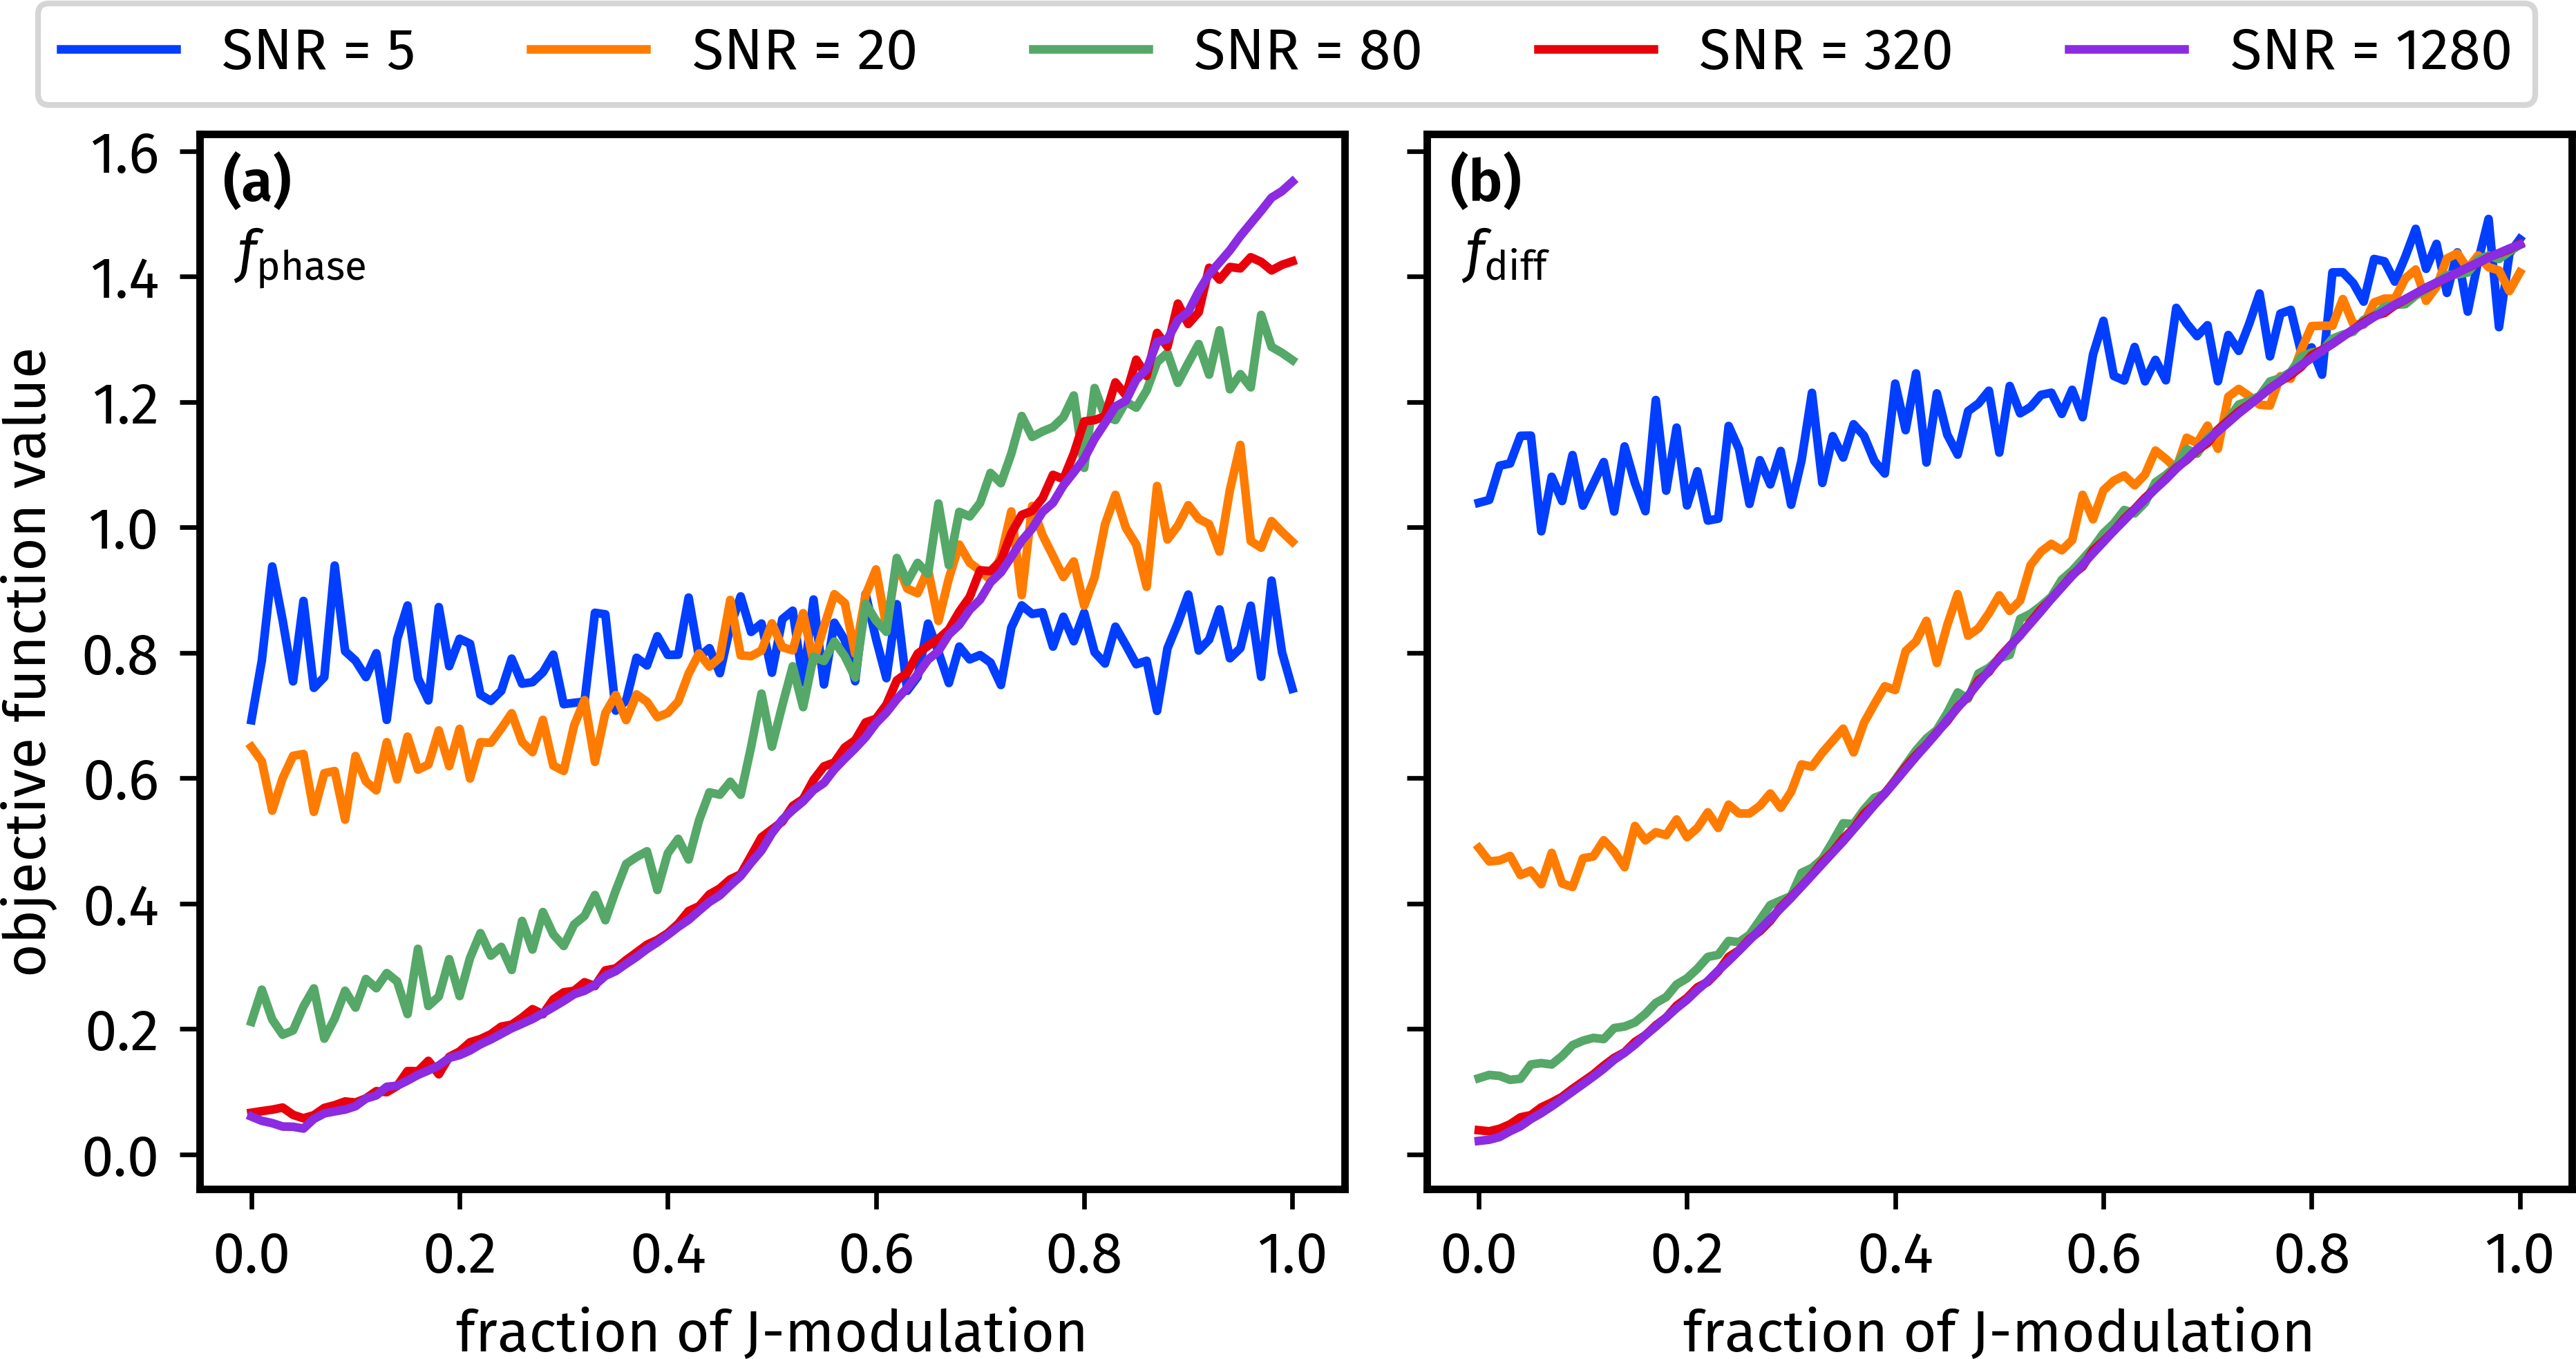
\includegraphics[]{pureshift/fa_scan_synthetic.png}
    {\phantomsubcaption\label{fig:fa_scan_synthetic_fphase}}
    {\phantomsubcaption\label{fig:fa_scan_synthetic_fdiff}}
    \caption[Evaluation of $f_\text{phase}$ and $f_\text{diff}$ cost functions on synthetic data]{
        Behaviour of the two cost functions, $f_\text{phase}$ and $f_\text{diff}$, on synthetic spectra with various SNRs.
        Zero phase distortion refers to an in-phase absorption-mode doublet, whereas complete phase distortion refers to an antiphase dispersion-mode doublet.
        \textbf{(\subref{fig:fa_scan_synthetic_fphase})} The $f_\text{phase}$ cost function.
        \textbf{(\subref{fig:fa_scan_synthetic_fdiff})} The $f_\text{diff}$ cost function, measured against a spectrum with no phase distortion and an SNR of 500.
    }
    \label{fig:fa_scan_synthetic}
\end{figure}

These two cost functions were chosen as they exhibited desirable characteristics on synthetic data (\cref{fig:fa_scan_synthetic}).
In these simulations, the `target' spectrum was chosen to simply be an in-phase absorption-mode doublet with an SNR of 500.
Synthetic data with increasing amounts of phase distortion (i.e.\ spectra ranging from in-phase absorption, to antiphase dispersion) were generated, and extra Gaussian noise added to create different SNRs.
It can be seen that, for data which is well-phased (left edges of the plots), both $f_\text{phase}$ (\cref{fig:fa_scan_synthetic_fphase}) and $f_\text{diff}$ (\cref{fig:fa_scan_synthetic_fdiff}) penalise lower SNRs.
Furthermore, both of the cost functions penalise phase distortions in multiplets, since they increase going from left to right.
This penalty is stricter for high-SNR spectra, which is also desirable, since it is only in high-SNR spectra that the phase distortions become noticeable.

The cost function $f_\text{diff}$ is easier to comprehend: it simply scales both the target and PSSE spectra down by their respective intensities, and compares each point to determine whether the peak shapes obtained are similar.
Although this seems like it should be agnostic towards signal intensity, this is only true for noiseless spectra.
If a (genuine) PSSE spectrum has low SNR, $\lVert \symbf{S}_\text{re} \rVert$ will be small, and the noise will be scaled down less than for the target spectrum; this difference in the noise then contributes towards the cost function.
On the other hand, a proper rationalisation of why the cost function $f_\text{phase}$ works is unfortunately not within my capabilities!
It was mostly developed by trial-and-error (based on the notion that phase distortions would have something to do with $\symbf{S}_\text{re}$ and $\symbf{S}_\text{im}$), and I do not have a good explanation of why it works.

\begin{figure}[htbp]
    \centering
    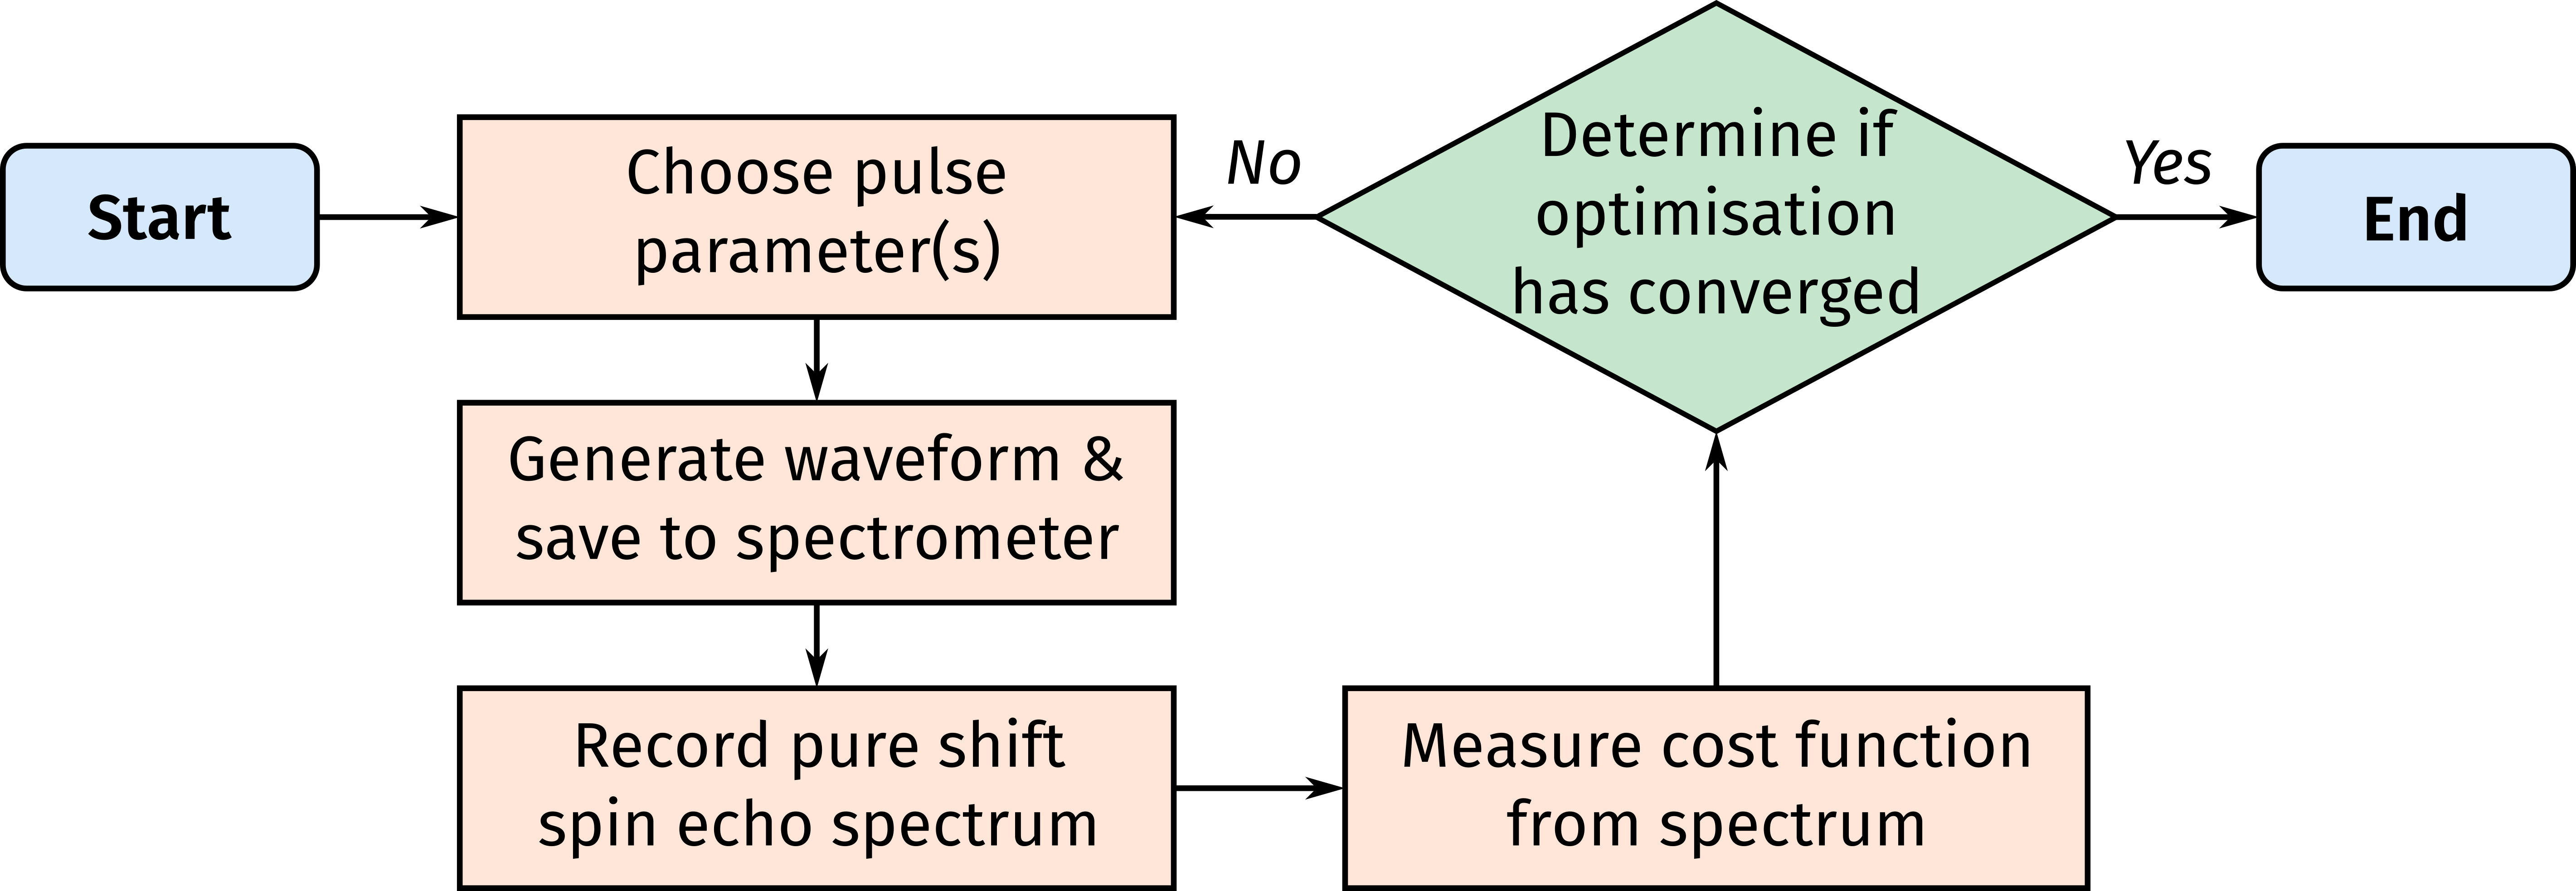
\includegraphics[]{pureshift/optim_flowchart_early.png}
    \caption[Flowchart for pure shift optimisation process]{
        Flowchart illustrating the steps for optimisation of a pure shift spectrum.
    }
    \label{fig:optim_flowchart_early}
\end{figure}

The general optimisation procedure is conceptually simple and largely consists of the loop shown in \cref{fig:optim_flowchart_early}: this is essentially a specialised version of the POISE flowchart (\todo{CREF TO FIG}).
The optimisation algorithm is responsible for determining convergence, as well as choosing the new parameters based on previously obtained information; the initial parameters must be supplied by the user.

In practice, it is a technical challenge to implement this loop on a spectrometer as the cost function calculation is performed either in Matlab or Python 3, both of which are not compatible with Bruker's TopSpin software.
TopSpin instead provides Jython (Python 2.7) and C programming interfaces;%
\footnote{TopSpin 4.1.4 introduced a Python 3 interface which would have made much of this work simpler. Unfortunately, this was not available at the time of this work.}
the former is not compatible with Python 3 packages like \texttt{numpy} or \texttt{scipy}, and the latter is too low-level to be worth implementing numerical algorithms in.%
\footnote{Of course, heavily optimised code in low-level languages such as C and Fortran---or perhaps even Matlab---would run faster. However, speeding up the code has virtually no impact on the optimisation, since its rate is limited by spectrum acquisition. In this situation, it makes far more sense to save \textit{developer time}.}
Thus, we require a means of \textit{communication} between the spectrometer and the optimisation control programme: this includes a signal from the controlling programme to trigger acquisition on the spectrometer, as well as a signal from the spectrometer that acquisition is done so that the cost function can be calculated.
As it turns out, the code used for the optimisations in this section was a very rudimentary and fragile form of that eventually used in POISE (for example, the aforementioned signals were transmitted via the creation and deletion of files).
I therefore defer the discussion of this issue to \cref{sec:poise__implementation}, where the more robust POISE interface is explained in detail.

\subsection{Flip angle optimisation}
\label{subsec:pureshift__faopt}

Having described the rest of the optimisation setup, it remains to choose exactly which parameters are subjected to optimisation.
The simplest option is to only optimise one parameter, namely the flip angle of the (double-)saltire pulse.
The flip angle dependence of PSYCHE spectra is well-understood, which crucially allows us to evaluate the cost functions outlined above and determine whether they are functioning correctly.

I first sought to measure how the cost functions described above varied with the flip angle.
To this end, pure shift spin echo spectra using a \textit{single} saltire as the PSE and various flip angles (from \ang{4} to \ang{50}) were acquired.
Since both cost functions penalise both low sensitivity and low purity, we expected that there would be an intermediate value where neither sensitivity nor purity were penalised too much: this would the optimum to seek.
In the event, it was found that only $f_\text{diff}$ yielded a useful minimum at around \ang{30} (albeit only a very shallow one, \cref{fig:fa_scan_cyclo}).

\begin{figure}[htb]
    \centering
    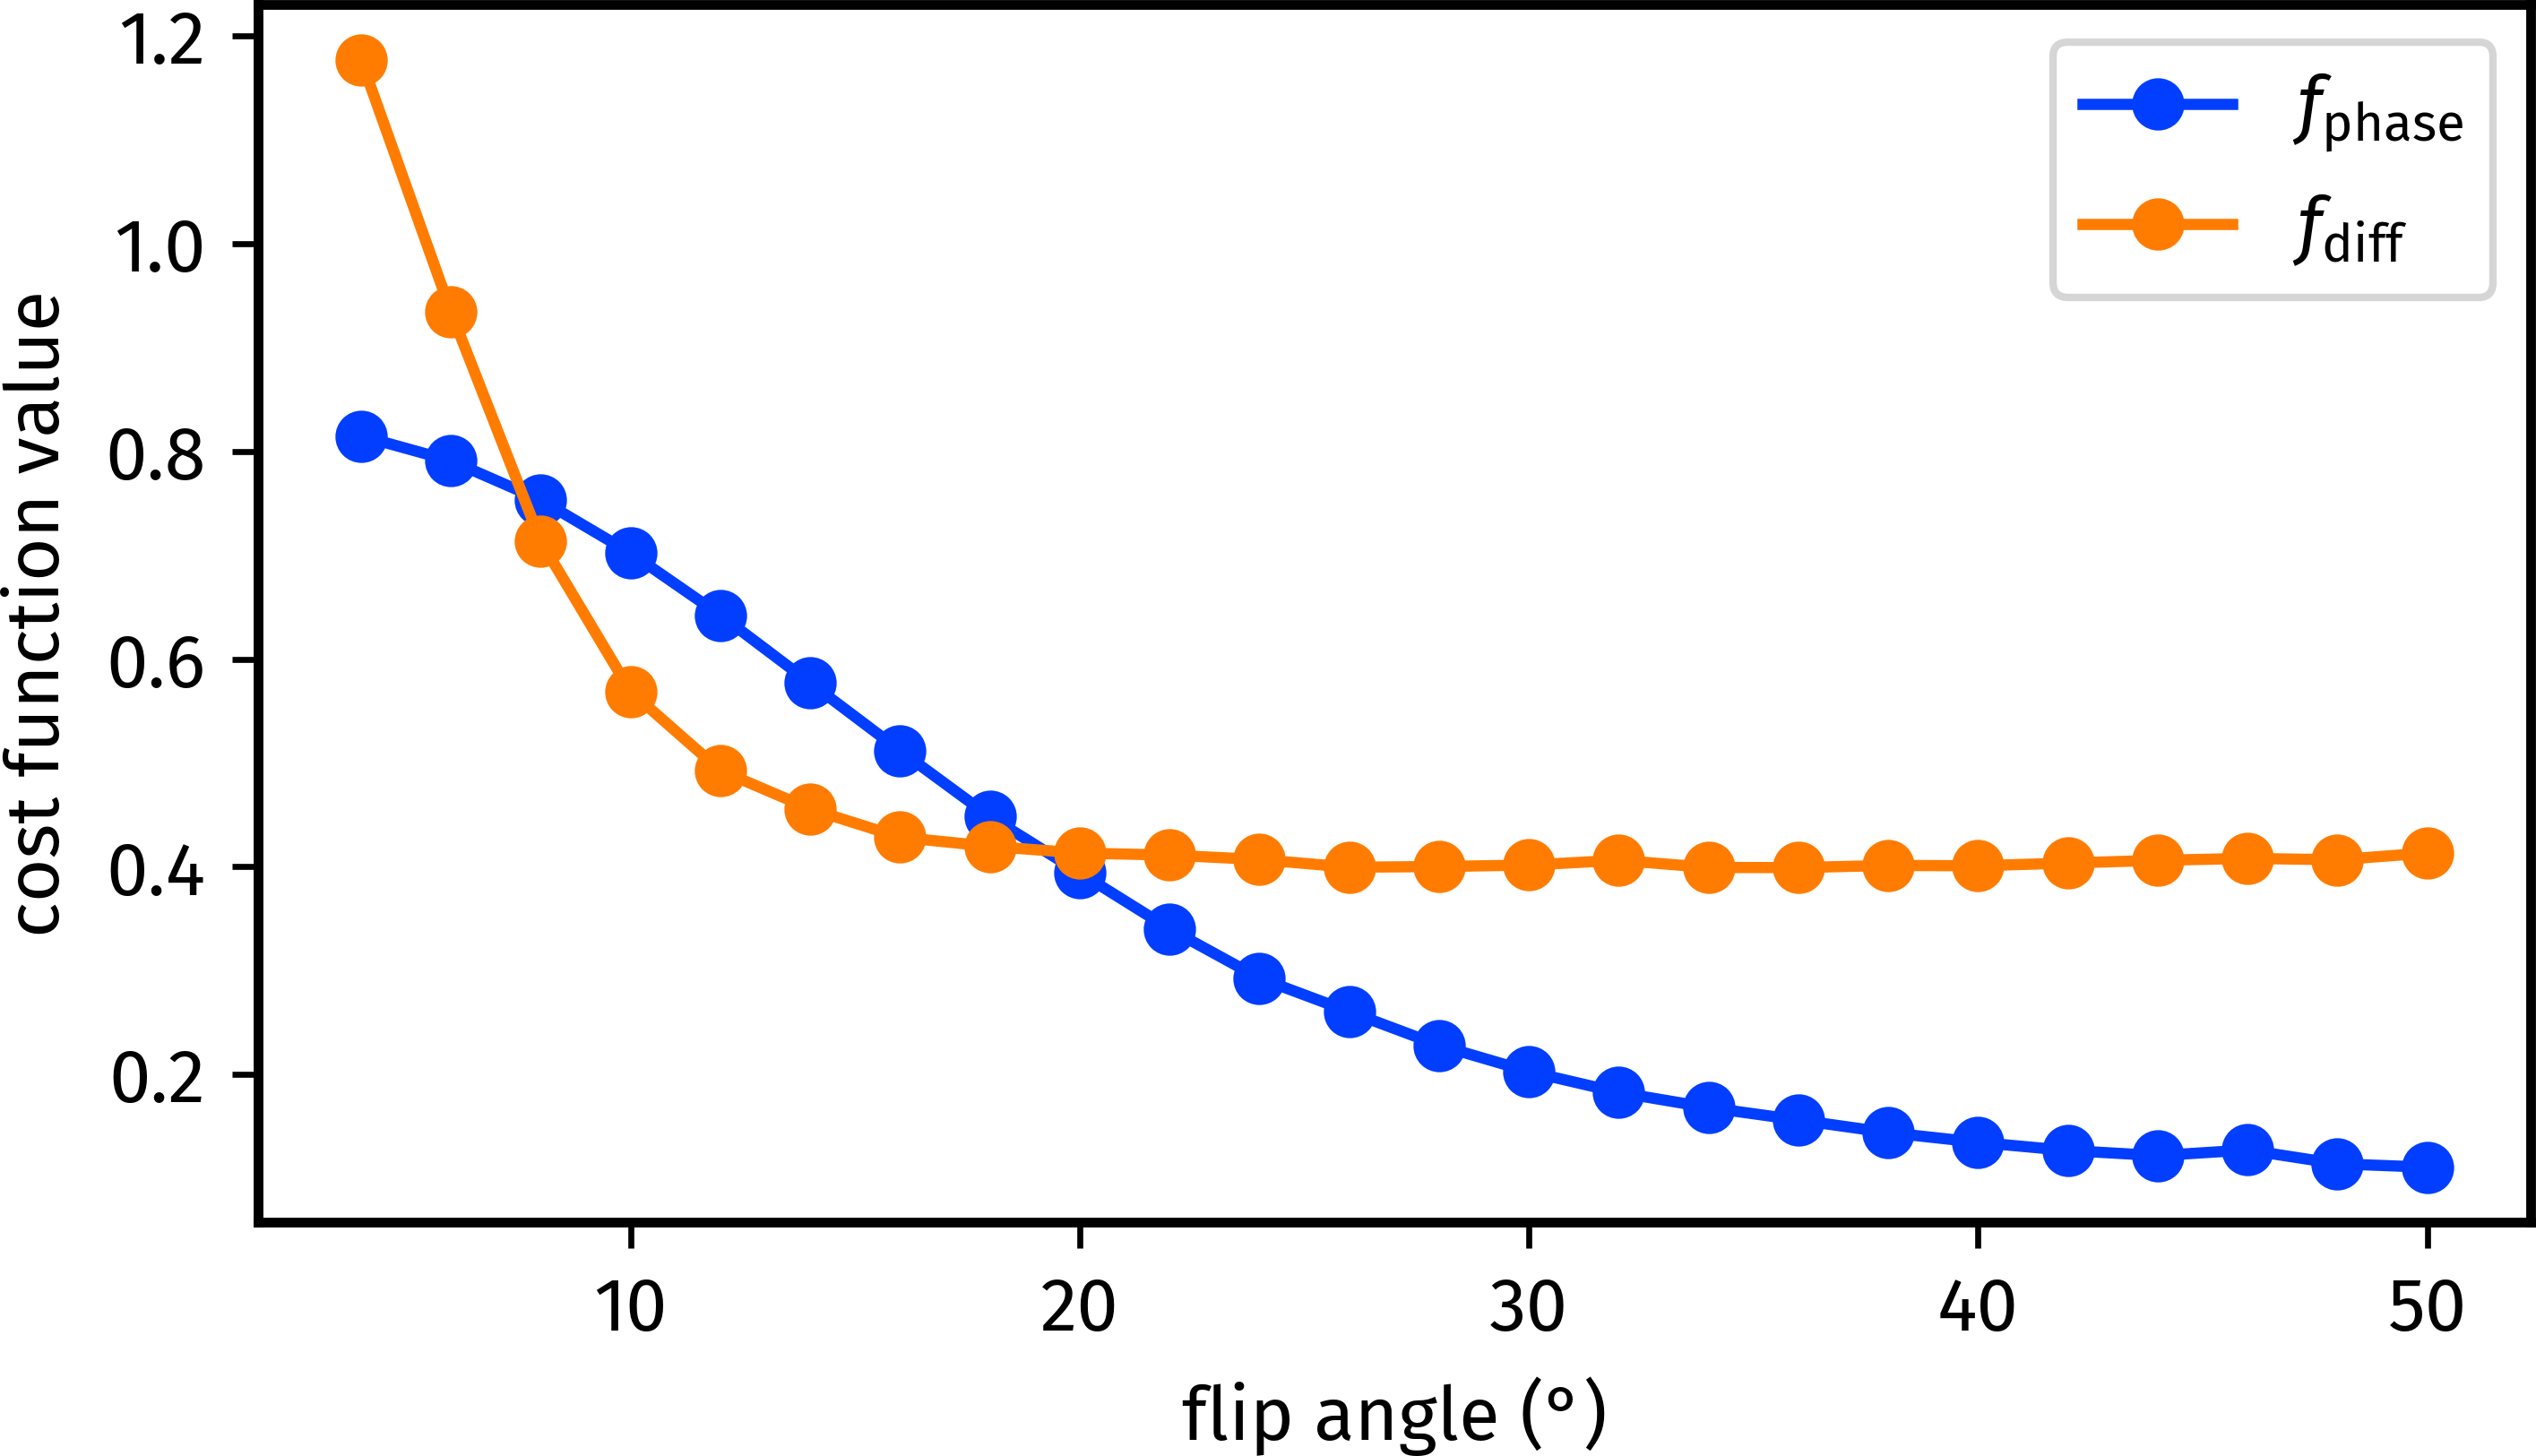
\includegraphics[draft=false]{pureshift/fa_scan_cyclo.png}
    \caption[Behaviour of $f_\text{phase}$ and $f_\text{diff}$ on experimental pure shift spin echo spectra.]{
        Behaviour of the two cost functions, $f_\text{phase}$ and $f_\text{diff}$, on experimental pure shift spin echo spectra.
        \datacode{6C-190907}
    }
    \label{fig:fa_scan_cyclo}
\end{figure}

\todo{
\begin{itemize}
    \item Explain `why' the two cost functions work (we can only really explain it for specdiff, not phase)
    \item Note that specdiff works almost by coincidence --- why does it have that exact balance of sensitivity vs purity? It could easily be something else. Note that this has not much relation to quality of pure shift spectra.
    \item Briefly mention that optimisations were done and converged to minimum as shown in plot --- no need to go into ynamide optimisations as the \ang{70} result is dubious
\end{itemize}
}

\subsection{Waveform parameterisation and optimisation}
\label{subsec:pureshift__chirpopt}

Given that a working optimisation setup, including cost functions, had been developed, it was a logical step to then test it out on a more challenging problem: namely, how the waveform used in the PSYCHE PSE could be modified.
This goes beyond simply modifying the number of saltires, as was done in \cref{sec:pureshift__nsaltire}.
There is no real reason why the pulse \textit{must} be an integer number of saltires: in principle it can have \textit{any} shape, although being symmetric about the centre of the pulse would likely still be beneficial in terms of preserving the mechanism of spatiotemporal averaging.

A naive attempt at optimising the pulse would simply involve modifying every pulse point in the double-saltire waveform used in the PSYCHE element.
As described in \cref{sec:theory__rotating_frame}, each pulse point consists of a pair of $x$- and $y$-amplitudes $(c_x, c_y)$; therefore, for a pulse with $n$ points, we would have a parameter vector $\symbf{x} \in \mathbb{R}^{2n}$.
Unfortunately, for PSYCHE, $n$ is on the order of $10000$, and an optimisation with $20000$ points is totally unfeasible.%
\footnote{Although problems of this size have been tackled using optimal control theory\autocite{Khaneja2005JMR,deFouquieres2011JMR,Glaser2015EPJD,Goodwin2016JCP}, it is not really feasible to use it in cases where the pulse is applied \textit{together} with a gradient, as is the case in PSYCHE. On top of that, the coupling networks and spin systems of interest are rather more complicated than in typical applications of optimal control.}

As a result of this, we must consider other ways of parameterising the waveform.
Several approaches to this issue have surfaced in the literature, such as the use of Fourier series\autocite{Geen1991JMR,Kupce1995JMRSB}, Gaussian cascades\autocite{Emsley1990CPL}, or spline interpolation between a subset of pulse points\autocite{Ewing1990CP}.
In this instance, we can use the knowledge that the PSYCHE PSE is composed of saltire pulses to our advantage.
Each saltire pulse is a linear combination of two chirps, defined by:
\begin{align}
    \phi(t) &= \phi_0 + \pi\taup(\Delta F)\left(\frac{t}{\taup} - \frac{1}{2}\right)^2 \label{eq:chirp_pulse_phase} \\
    c_x(t) &= A \cos[\phi(t)] \label{eq:chirp_pulse_cx} \\
    c_y(t) &= A \sin[\phi(t)] \label{eq:chirp_pulse_cy}
\end{align}
for $t \in [0, \taup]$. Here, $\taup$ is the duration of the chirp, $A$ is the amplitude of the chirp (which is time-independent), $\phi_0$ the phase of the chirp, and $\Delta F$ the bandwidth.
(Note that \cref{eq:chirp_pulse_cx,eq:chirp_pulse_cy} are identical to \cref{eq:pulse_cartesian}.)

\begin{figure}[htb]
    \centering
    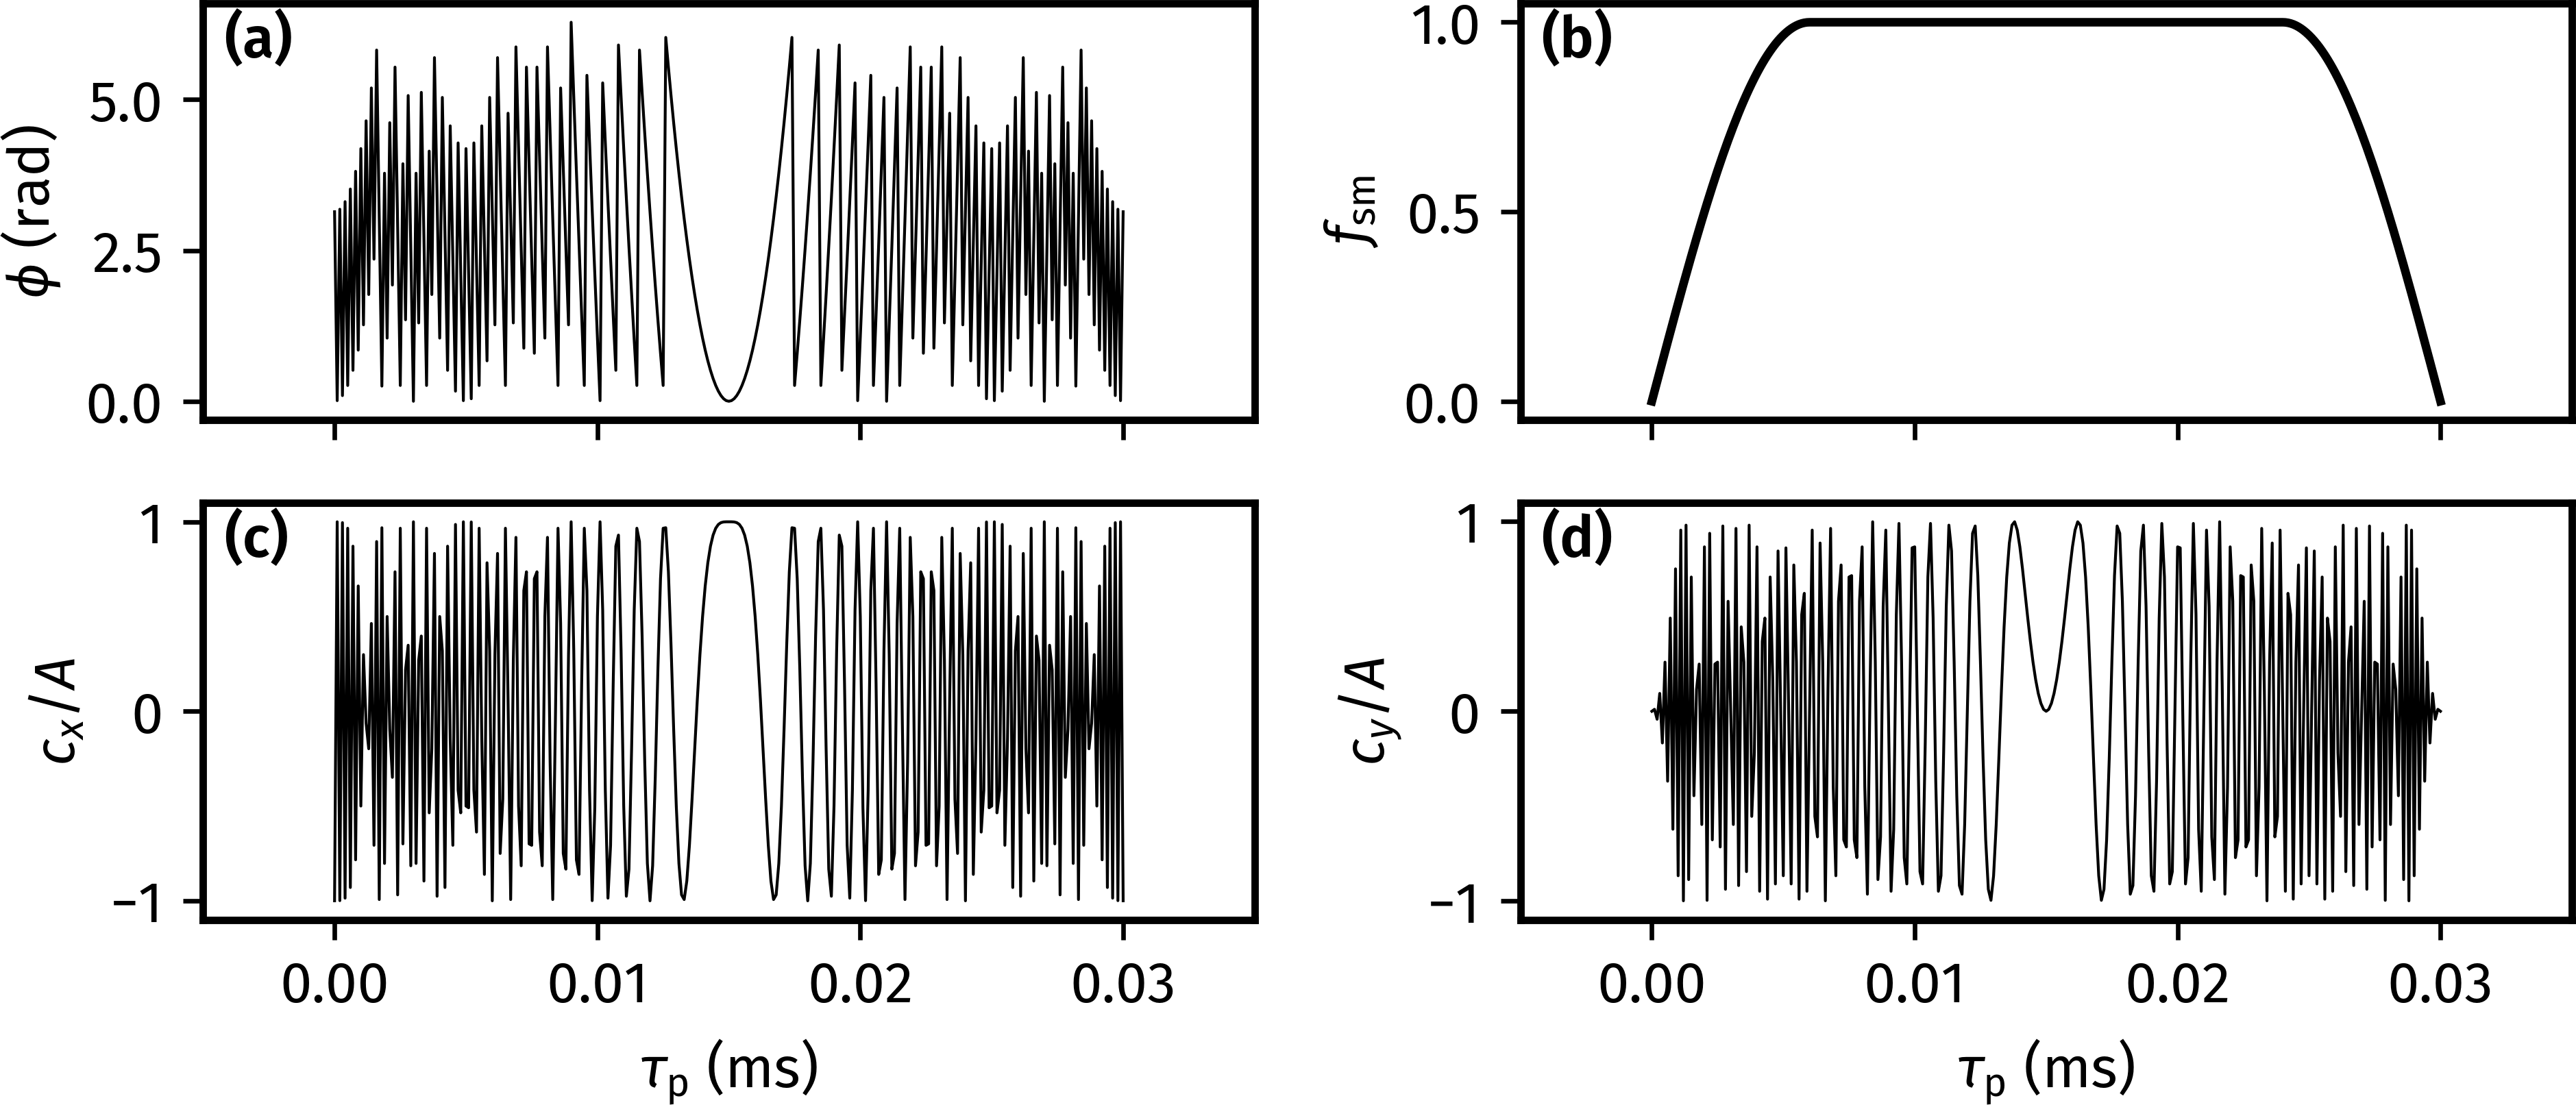
\includegraphics[]{pureshift/chirp_coefficients.png}
    {\phantomsubcaption\label{fig:chirp_coefficients_phase}}
    {\phantomsubcaption\label{fig:chirp_coefficients_smoothing}}
    {\phantomsubcaption\label{fig:chirp_coefficients_cx}}
    {\phantomsubcaption\label{fig:chirp_coefficients_cy}}
    \caption[Phase and Cartesian amplitudes of a typical chirp pulse]{
        Plots of the quantities in \cref{eq:chirp_pulse_phase,eq:chirp_pulse_cx,eq:chirp_pulse_cy} for a typical chirp pulse ($\taup = \SI{30}{\ms}$, $\Delta F = \SI{10}{\kHz}$).
        \textbf{(\subref{fig:chirp_coefficients_phase})} $\phi(t)$ wrapped to the range $[0, 2\pi)$.
        \textbf{(\subref{fig:chirp_coefficients_smoothing})} The quarter-sine smoothing profile which is later applied to the entire waveform (\cref{eq:sming_function}); here $s_\text{sm} = 0.2$.
        \textbf{(\subref{fig:chirp_coefficients_cx})} $c_x(t)/A$ prior to smoothing.
        \textbf{(\subref{fig:chirp_coefficients_cy})} $c_y(t)/A$ prior to smoothing.
        The amplitude $A$ is simply a constant which reflects the flip angle of the chirp.\autocite{Foroozandeh2018CEJ}
    }
    \label{fig:chirp_coefficients}
\end{figure}

Given these expressions, we see that there are four parameters of the chirp which can be modified: $A$, $\taup$, $\phi_0$, and $\Delta F$.
The two chirps which form one saltire pulse simultaneously sweep in opposite directions, which mean that $\Delta F$ for one chirp is the negative of the other; however, their parameters are otherwise equal.
We may, however, also envision a case where the pulse is constructed from two chirps which are applied at a different point in time, and also cover different bandwidths.
This adds two more parameters to each chirp, namely $t_0$ (the starting time of the pulse) and $f_0$ (the centre of the pulse bandwidth).
Each chirp therefore sweeps from the frequency $f_0 - (\Delta F)/2$ at a time $t_0$, to the frequency $f_0 + (\Delta F)/2$ at a time $t_0 + \taup$.
In total, this gives us six parameters per chirp which may be optimised: for a sum of two chirps, there are therefore 12 parameters in total.

Since a sum of two chirps is not necessarily symmetric (with respect to reflection in time), I opted to reflect the waveform about its end, thus doubling the length of the pulse.
The entire waveform was then multiplied by a \textit{smoothing function} $f_\text{sm}(t)$ (\cref{fig:chirp_coefficients_smoothing}), which prevents large jumps in RF amplitude at the beginning and end of the pulse.
$f_\text{sm}$ depends on a smoothing parameter $s_\text{sm}$, which is typically $0.1$--$0.2$:
\begin{equation}
    \label{eq:sming_function}
    f_\text{sm}(t) = \begin{cases}
        \displaystyle \sin\left(\frac{\pi t'}{2 s_\text{sm}}\right) & 0 \leq t' < s_\text{sm}; \\
        \displaystyle 1 & s_\text{sm} \leq t' < 1 - s_\text{sm}; \\
        \displaystyle \sin\left[\frac{\pi (1 - t')}{2 s_\text{sm}}\right] & s_\text{sm} \leq t' \leq 1, \\
    \end{cases}
\end{equation}
where $t' = t/\taup$ (and here $\taup$ refers to the duration of the \textit{entire} waveform, after reflection.).

The initial point chosen was that corresponding to a single saltire after reflection:
\begin{itemize}
    \item Chirp 1: $\taup = \SI{15}{\ms}$; $\Delta F = \SI{-5}{\kHz}$; $\phi_0 = 0$; $A = \SI{36}{\Hz}$; $t_0 = 0$; $f_0 = \SI{5}{\kHz}$;
    \item Chirp 2: $\taup = \SI{15}{\ms}$; $\Delta F = \SI{5}{\kHz}$; $\phi_0 = 0$; $A = \SI{36}{\Hz}$; $t_0 = 0$; $f_0 = \SI{-5}{\kHz}$;
\end{itemize}
Collectively, these two pulses sum up to become the \textit{first half} of a single saltire with bandwidth $\SI{10}{\kHz}$.
After reflection, the total duration of the saltire is $\SI{30}{\ms}$, and the amplitude is $\SI{72}{\Hz}$, which corresponds to a flip angle of approximately \ang{32}.

\begin{figure}[htbp]
    \centering
    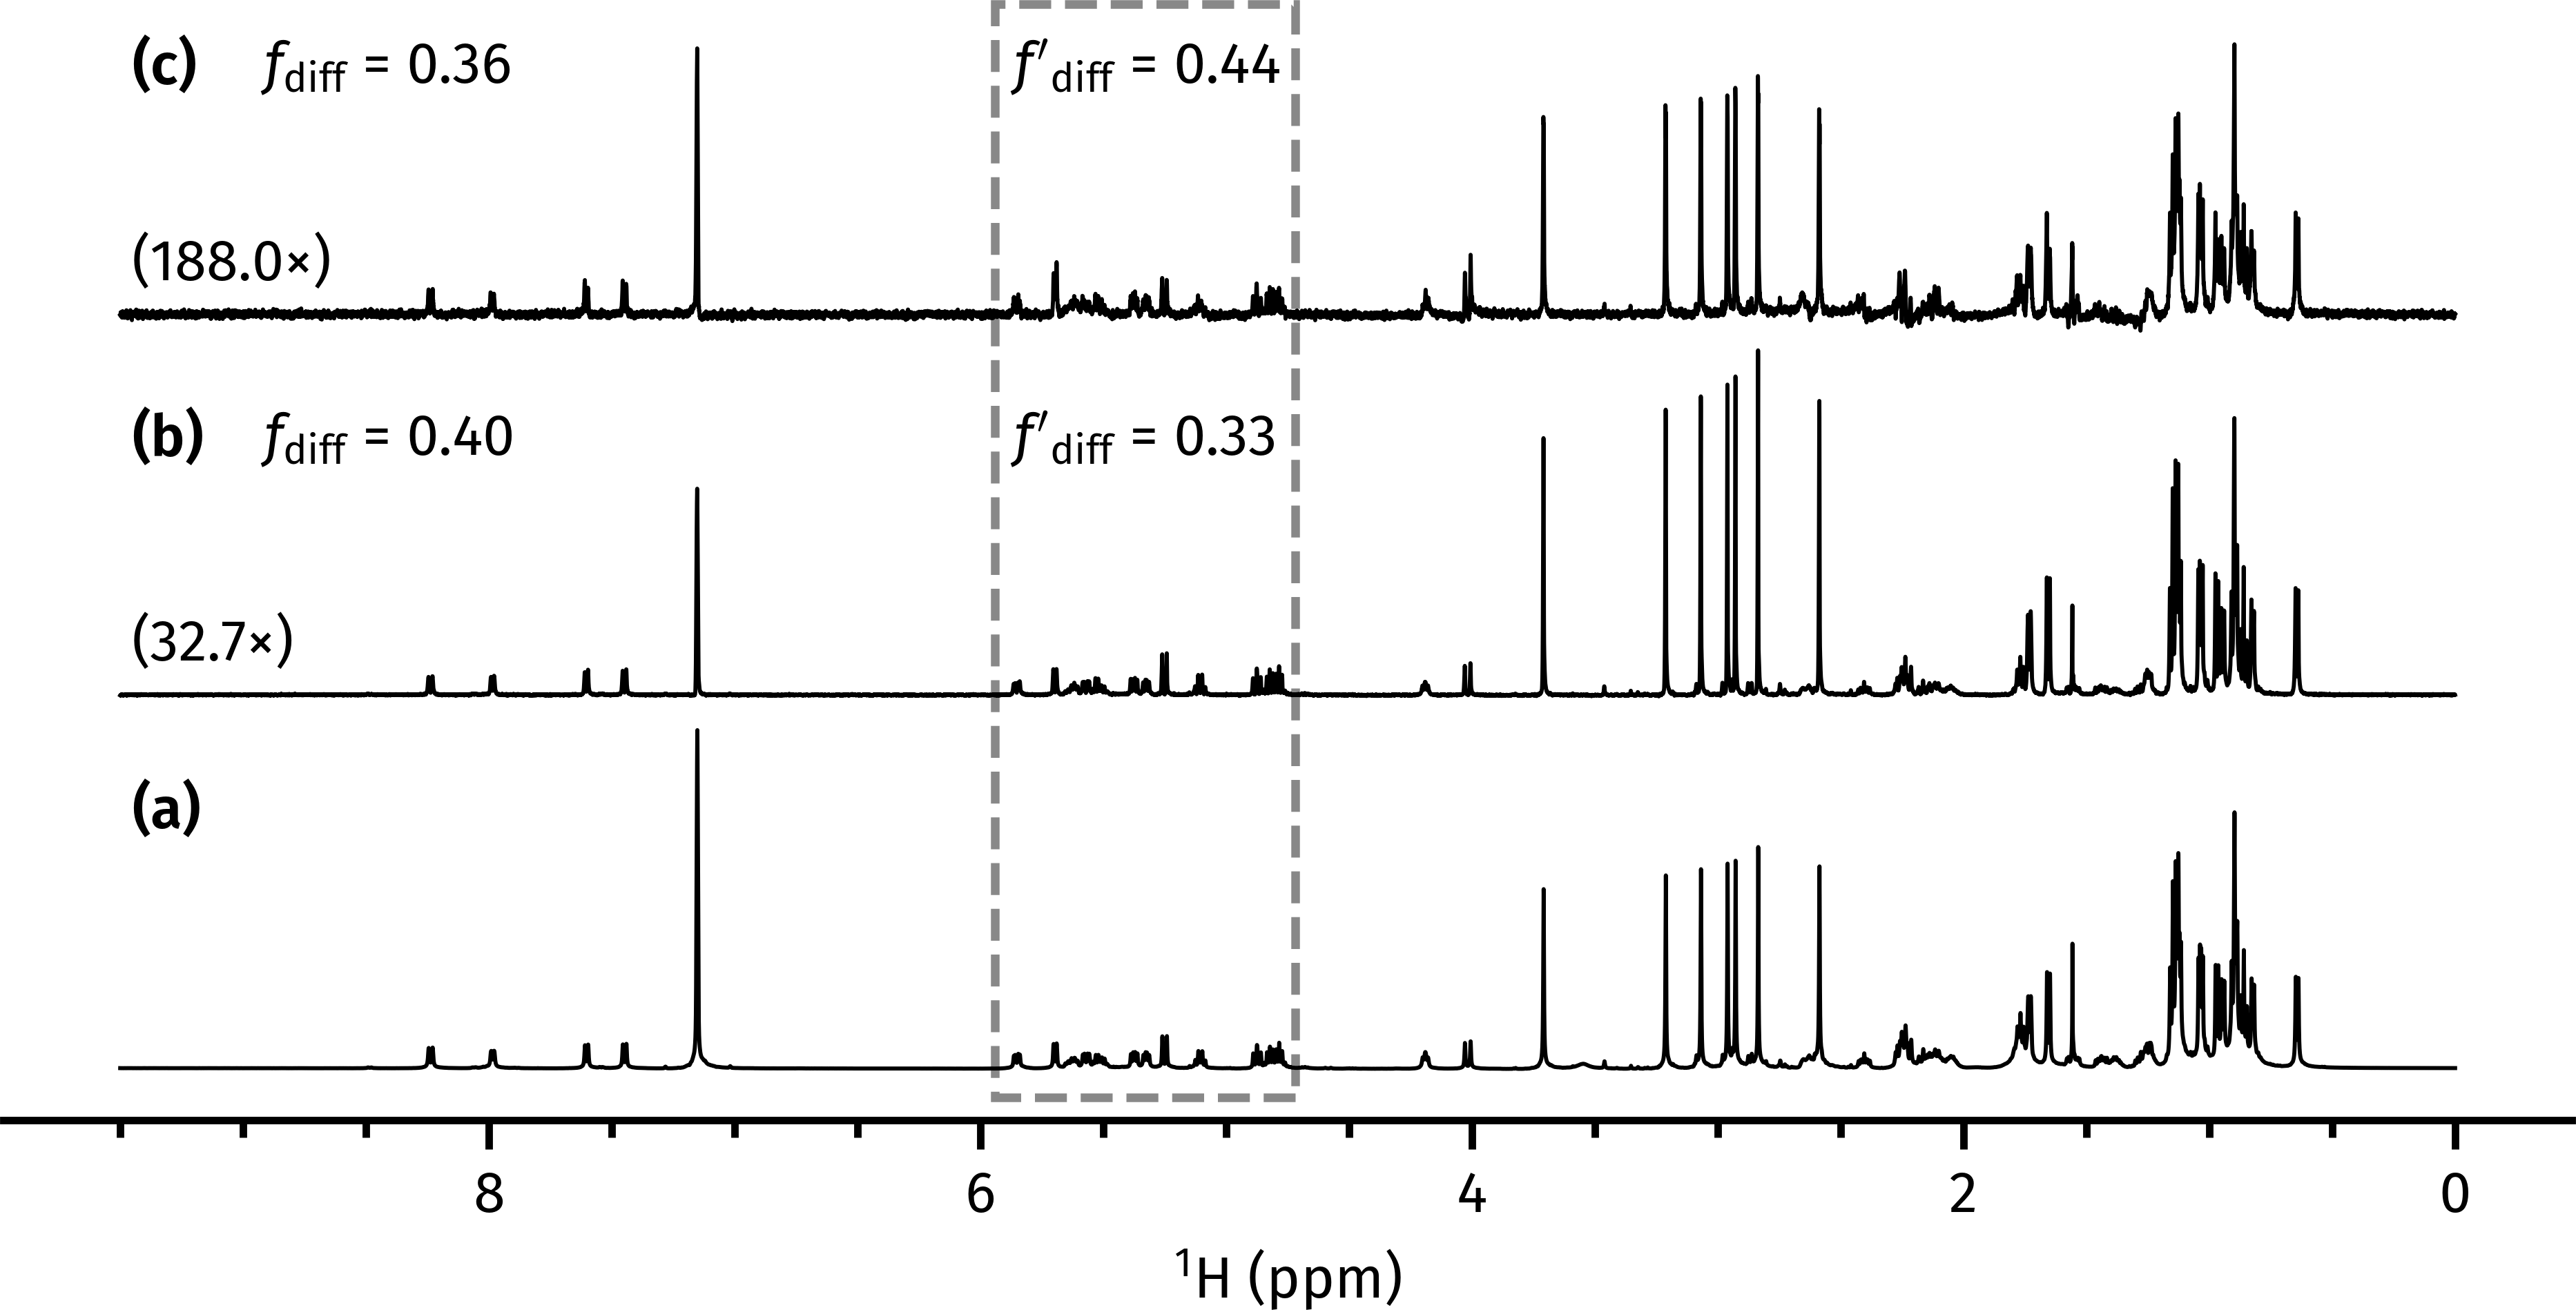
\includegraphics[]{pureshift/chirpopt_spurious.png}
    {\phantomsubcaption\label{fig:chirpopt_spurious_target}}
    {\phantomsubcaption\label{fig:chirpopt_spurious_saltire}}
    {\phantomsubcaption\label{fig:chirpopt_spurious_badoptimum}}
    \caption[Spurious optimum obtained in waveform optimisation using $f_\text{diff}$]{
        \textbf{(\subref{fig:chirpopt_spurious_target})} Target spectrum (pulse--acquire).
        \textbf{(\subref{fig:chirpopt_spurious_saltire})} PSSE spectrum obtained using the initial guess (a saltire).
        \textbf{(\subref{fig:chirpopt_spurious_badoptimum})} PSSE spectrum obtained with a spurious optimum point.
        The grey dotted box shows the restricted region over which $f_\text{diff}$ was subsequently applied to, yielding a formally different cost function $f'_\text{diff}$; this yielded more sensible results where the cost function for the saltire pulse was smaller.
        \datacode{6C-190823}
    }
    \label{fig:chirpopt_spurious}
\end{figure}

Using this setup, several optimisations of the 12 parameters above were conducted.
It was quickly noticed that, although $f_\text{diff}$ was a better cost function than $f_\text{phase}$, this led to spurious optima being located, such as the one in \cref{fig:chirpopt_spurious_badoptimum}.
Although the initial point (a saltire) yielded a much larger SNR (\cref{fig:chirpopt_spurious_saltire}), the value of $f_\text{diff}$ was still larger than for this false optimum.
The reason for this is almost certainly because the PSE distorts the relative intensity of the strong singlets in the spectrum, notably the $\ch{C6D5H}$ peak at \SI{7.15}{ppm}, and the \textit{N}-methyl groups between 2.5 and \SI{3.8}{\ppm}).

Of course, singlets are completely unimportant when devising a pure shift experiment.
Unfortunately, since singlets are typically more intense than the rest of the spectrum, they also contribute disproportionately to the cost function.
A simple and effective way to circumvent this is to restrict the part of the spectrum being evaluated.
In this case, I chose to use the $\ch{H}^{\alpha}$ region between 4.72 and \SI{5.94}{ppm} (grey dotted box in \cref{fig:chirpopt_spurious}).
This yields a formally different cost function, which I label as $f'_\text{diff}$.
With this, much more logical behaviour was observed: in particular, the saltire pulse performed better than the spurious optimum previously found.

While this new cost function could be successfully used to run optimisations, unfortunately most of these simply failed to find anything performing better than the original saltire pulse.
On the rare occasion where something `better' was found (as judged by the new cost function $f'_\text{diff}$), these were simply \textit{fairly close} to that of a saltire, and the corresponding decreases in the cost function extremely small---suggesting that the `better' result may simply just have been due to noise in the cost function.
Nevertheless, these new `optima' \textit{did} function as perfectly serviceable PSEs: for example, \cref{fig:newpulse_tsepsyche} compares a TSE-PSYCHE spectrum obtained with an optimised pulse to one obtained with the single saltire pulse.
There is virtually no difference.
This is a meaningful result, as it demonstrates that $f'_\text{diff}$ is actually an accurate metric to determine the quality of a PSE (it is noisy, but this is inevitable in an experimentally measured cost function).
Unfortunately, although the pulse shape is shown in \cref{fig:newpulse_tsepsyche_newpulse}, the exact parameters which generated this pulse shape have been lost to time.

\begin{figure}[htb]
    \centering
    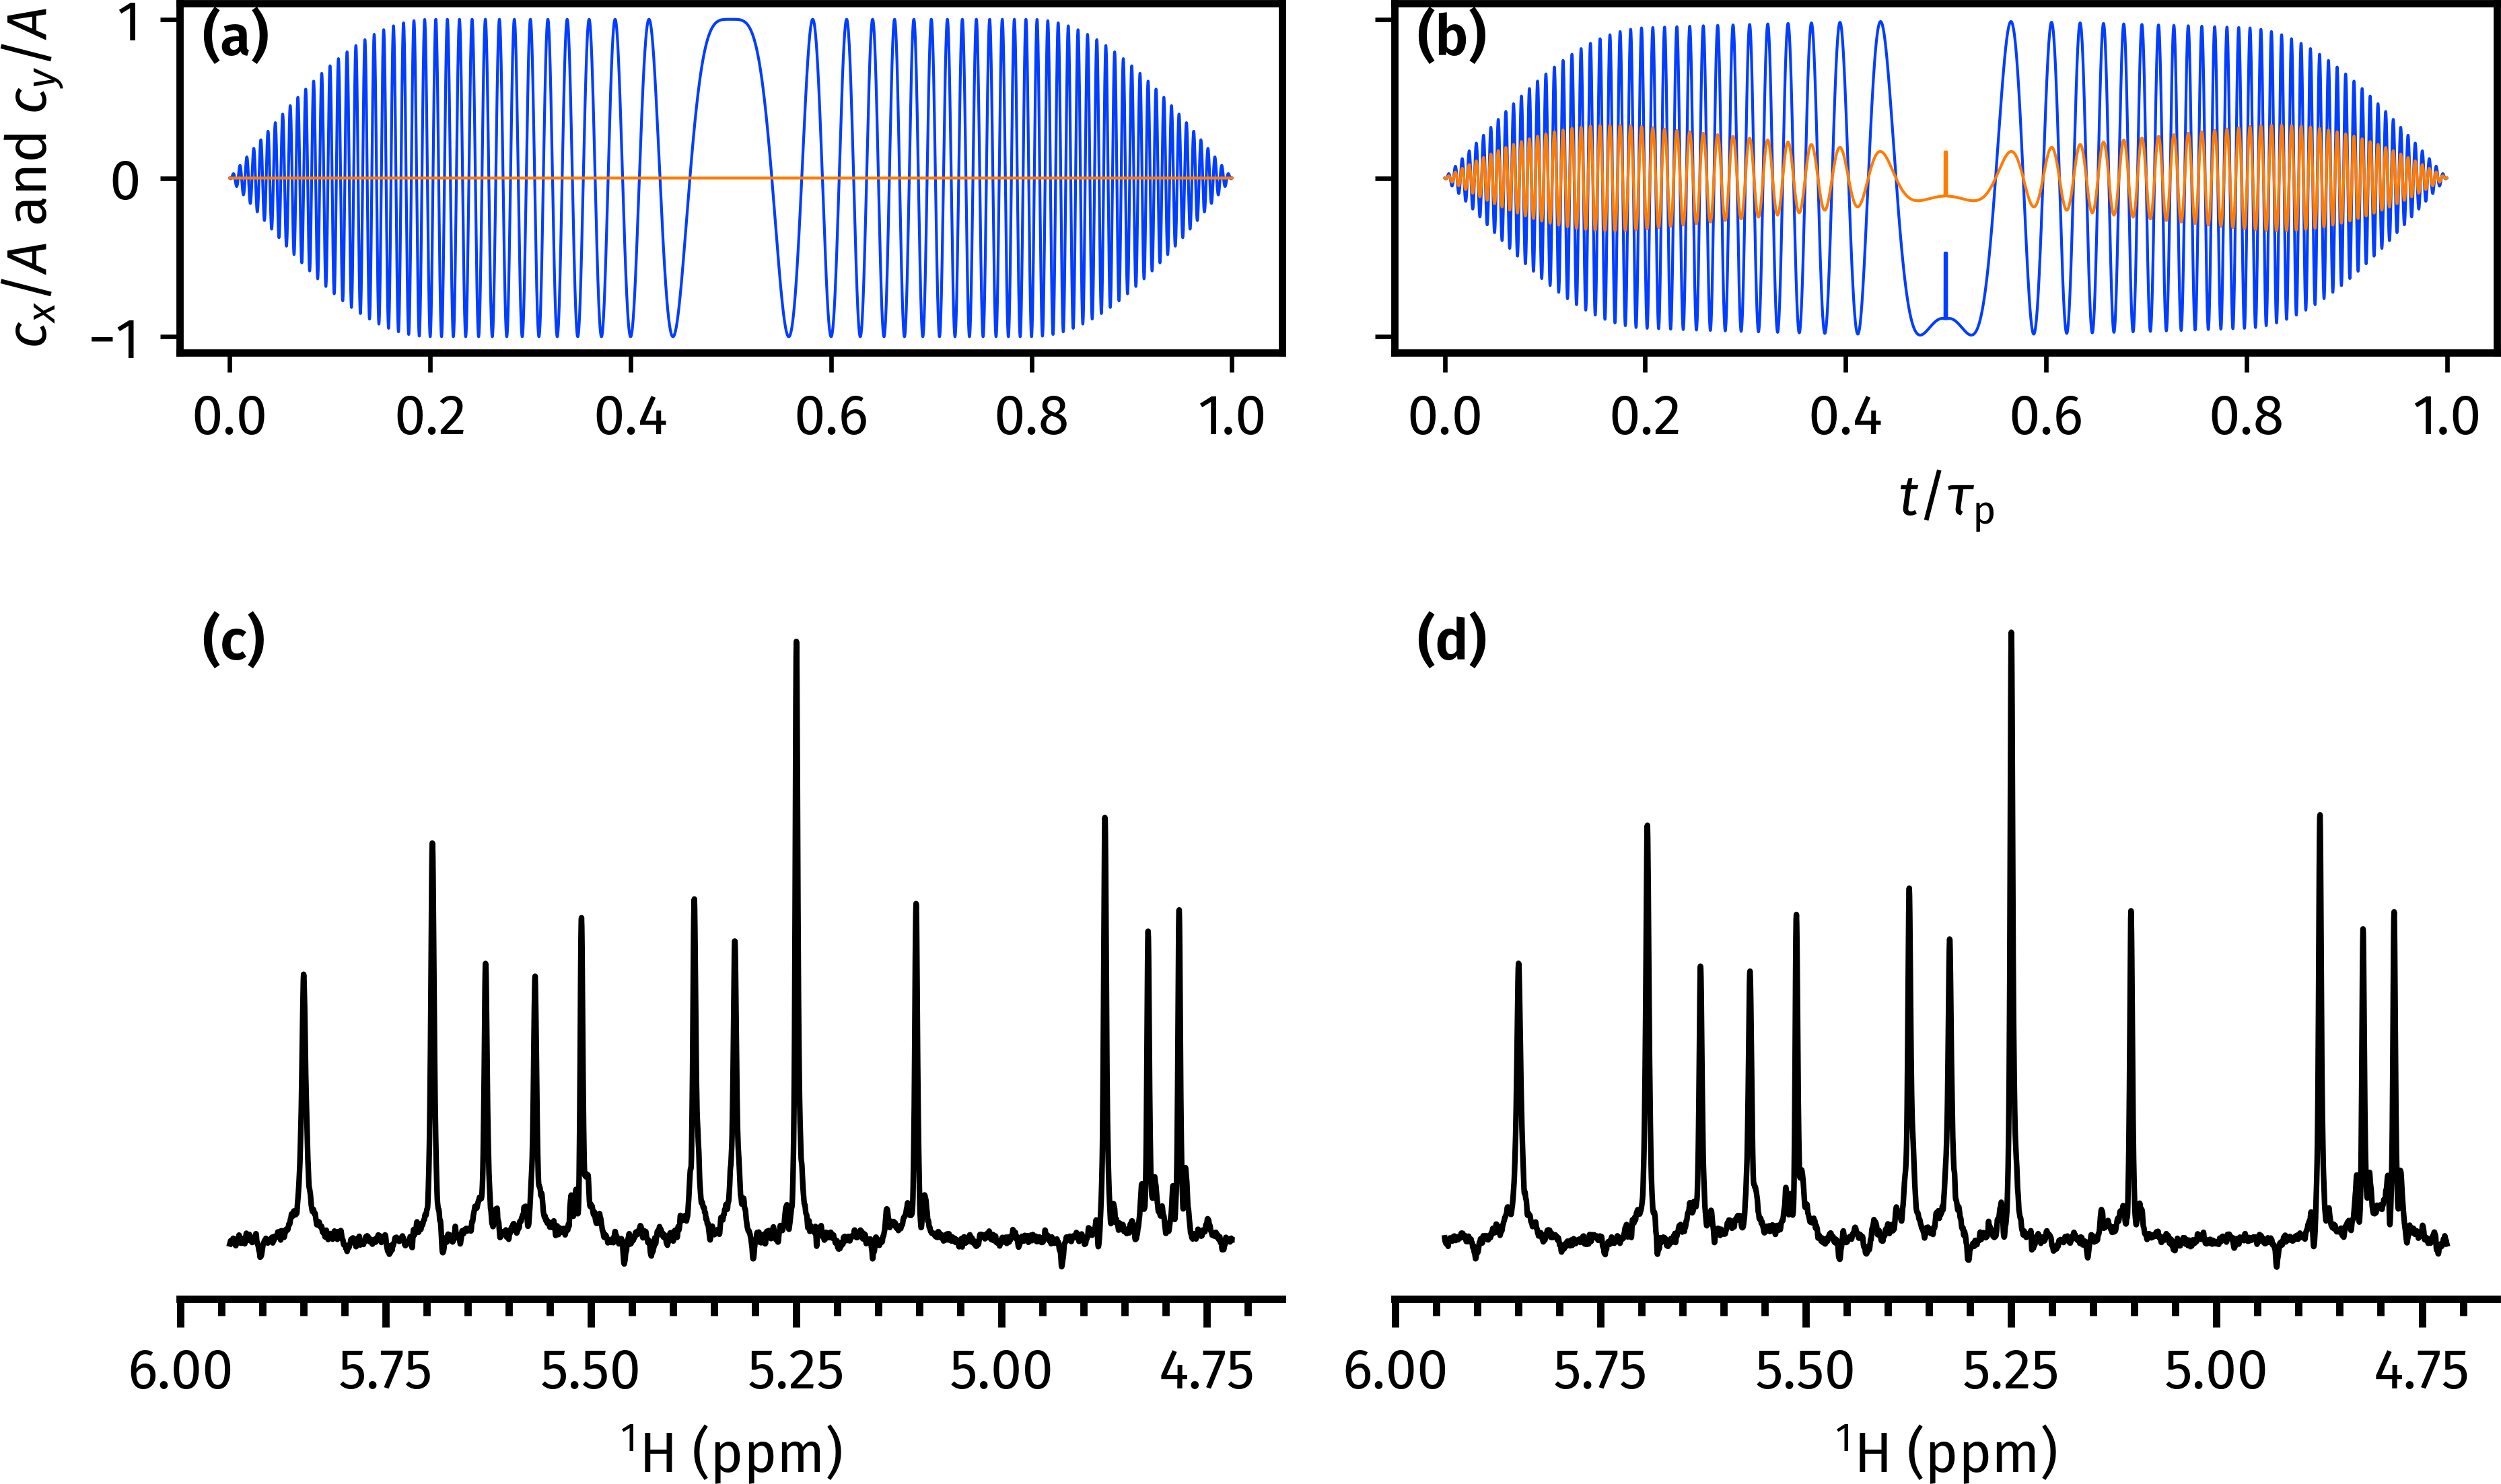
\includegraphics[]{pureshift/newpulse_tsepsyche.png}
    {\phantomsubcaption\label{fig:newpulse_tsepsyche_saltire}}
    {\phantomsubcaption\label{fig:newpulse_tsepsyche_newpulse}}
    {\phantomsubcaption\label{fig:newpulse_tsepsyche_saltirespec}}
    {\phantomsubcaption\label{fig:newpulse_tsepsyche_newpulsespec}}
    \caption[Evaluation of an `optimised' pulse in a TSE-PSYCHE experiment]{
        \textbf{(\subref{fig:newpulse_tsepsyche_saltire})} $x$- and $y$-coefficients of the initial saltire pulse (as a fraction of the maximum amplitude $A$).
        \textbf{(\subref{fig:newpulse_tsepsyche_newpulse})} $x$- and $y$-coefficients of the `optimised' pulse (as a fraction of the maximum amplitude $A$).
        \textbf{(\subref{fig:newpulse_tsepsyche_saltirespec})} TSE-PSYCHE spectrum obtained with the initial guess (a saltire pulse).
        \textbf{(\subref{fig:newpulse_tsepsyche_newpulsespec})} TSE-PSYCHE spectrum obtained with the `optimised' pulse, with virtually equivalent performance.
        \datacode{6C-190831}
    }
    \label{fig:newpulse_tsepsyche}
\end{figure}

In conclusion, while not quite as intractable as 20000 parameters, optimising a 12-parameter function clearly still proves to be a challenge.
Although the cost functions described here do work, they are generally quite `flat', in that they do not discriminate very sharply between `good' and `bad' spectra.
Combined with the fact that the cost function is noisy, this makes experimental optimisation of the waveform an uphill task.
Nevertheless, much of the knowledge (and code) in this section was later used in the development of POISE.
In the next two sections in this chapter, I will move on from PSYCHE and discuss completely different methods of obtaining pure shift spectra using only hard pulses in the PSE.

